% !TEX root = ../report.tex

\chapter{The SoBazar Data}
\minitoc
    This sections will introduce the Sobazar application and explore the Sobazar data set.
    This includes how the data was preprocessed, a summary of the dataset, statistics and graphs about the data and findings from the data.

	%Sobazar intro
	
	\section{Introduction to Sobazar}\mbox{}\\
	
	\begin{chapquote}[30pt]{About Sobazar}
	  "SOBAZAAR is a newly developed social shopping experience – a daily fashion bazaar on your mobile."
	\end{chapquote}
	
	Sobazar is an online marketplace for fashion, but with a social twist. The application lets you click through thousands of products. You can find stores like Moods of Norway, BIK BOK, Bianco and many more. If you find something you like you can purchase it directly from the application or store it for later with the \emph{love it} functionality. 
	The following screenshots are taken from the application and highlights some functionality currently found in the
	application.
		
	\begin{figure}[H]
		\centering
		\begin{minipage}{.30\linewidth}
	  		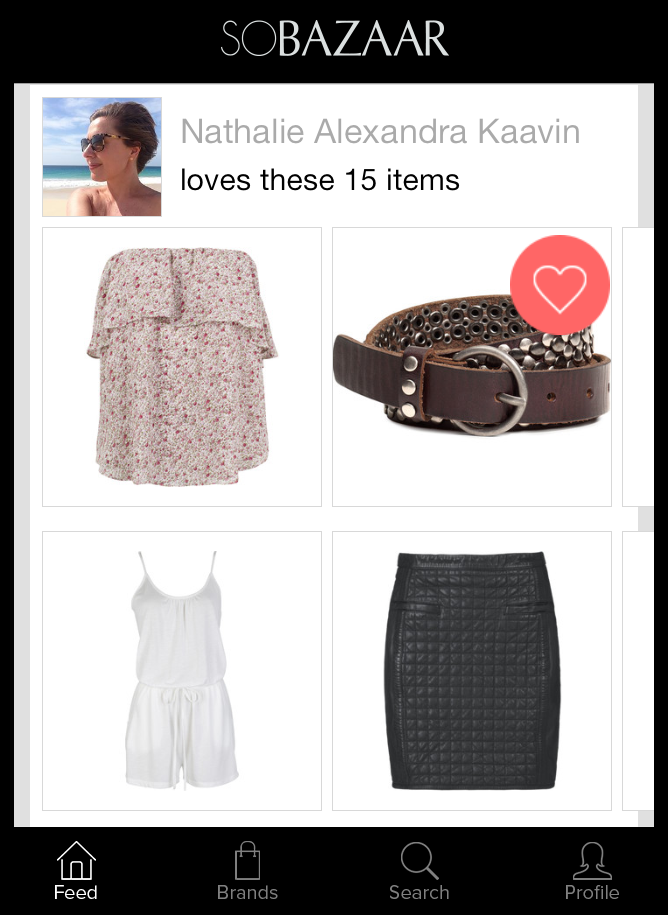
\includegraphics[height=1.5\linewidth]{image/sobazarfeed.png}
		\end{minipage}
		\hspace{.02\linewidth}
		\begin{minipage}{.30\linewidth}
			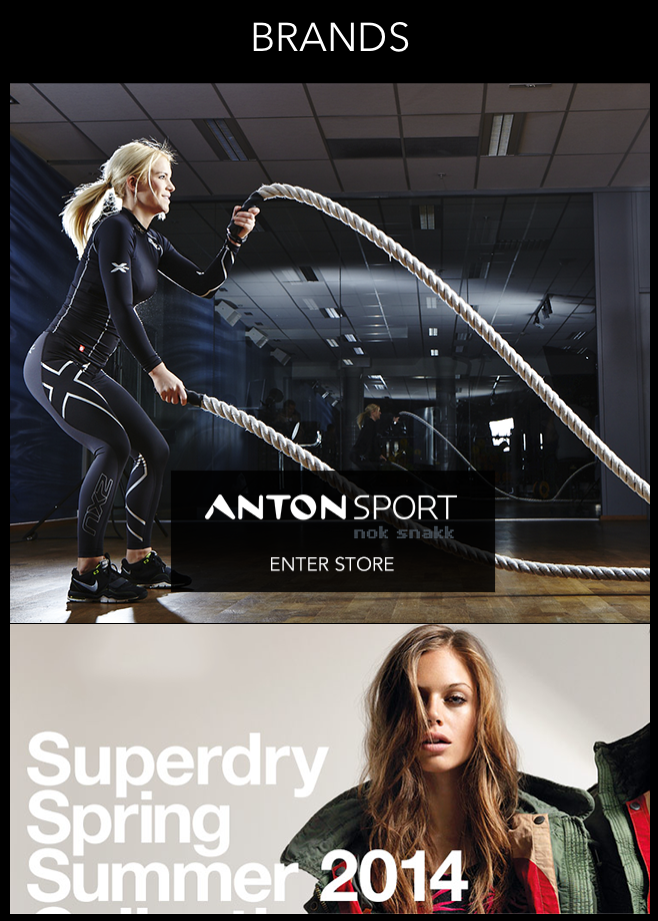
\includegraphics[height=1.5\linewidth]{image/sobazarbrands2.png} 
		\end{minipage}
		\hspace{.02\linewidth}
		\begin{minipage}{.30\linewidth}
			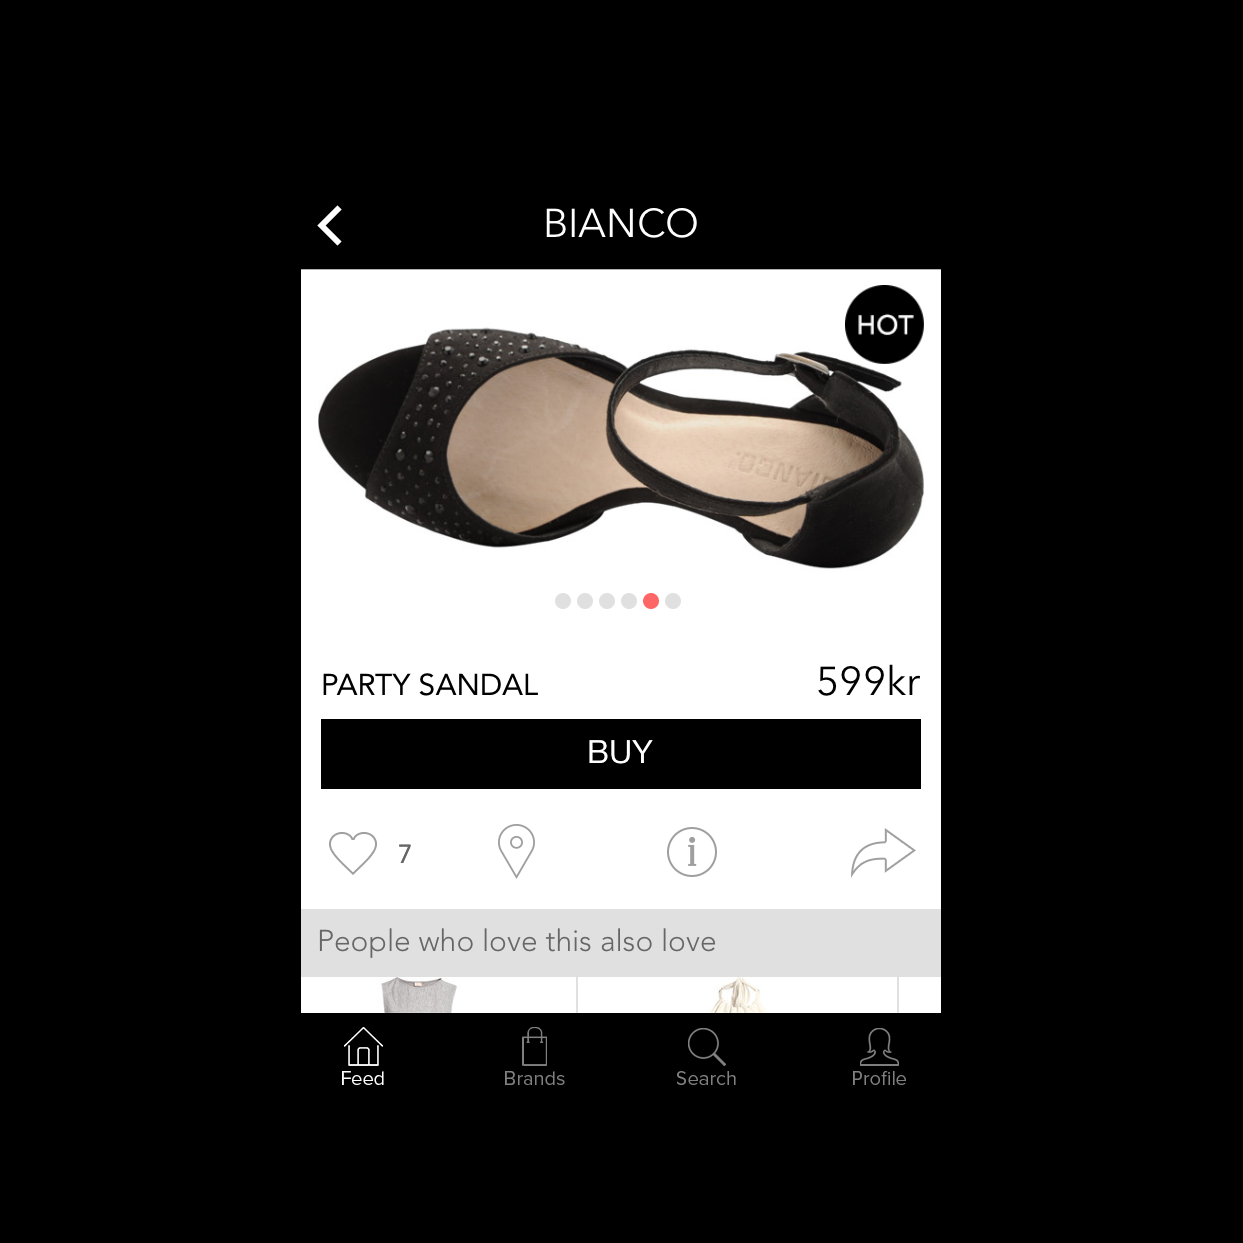
\includegraphics[height=1.5\linewidth]{image/sobazarproduct.png}
		\end{minipage}
		\caption[Sobazar screenshots - version 0.5.1]{Screenshots from the Sobazar Application. From the left to right: The Sobazar newsfeed, the brand browsing screen and the product screen}
		\label{figure:sobazarfeed}
	\end{figure}
	
	To help the customers find products the feed currently shows the activity of other users, notifies you about sales,
	presents the most popular items and the application also features an editors pick page among other things.
	The following screenshots show some functionality currently in place to help the customer find items to buy.
	
	\begin{figure}[H]
		\centering
		\begin{minipage}{.3\linewidth}
		  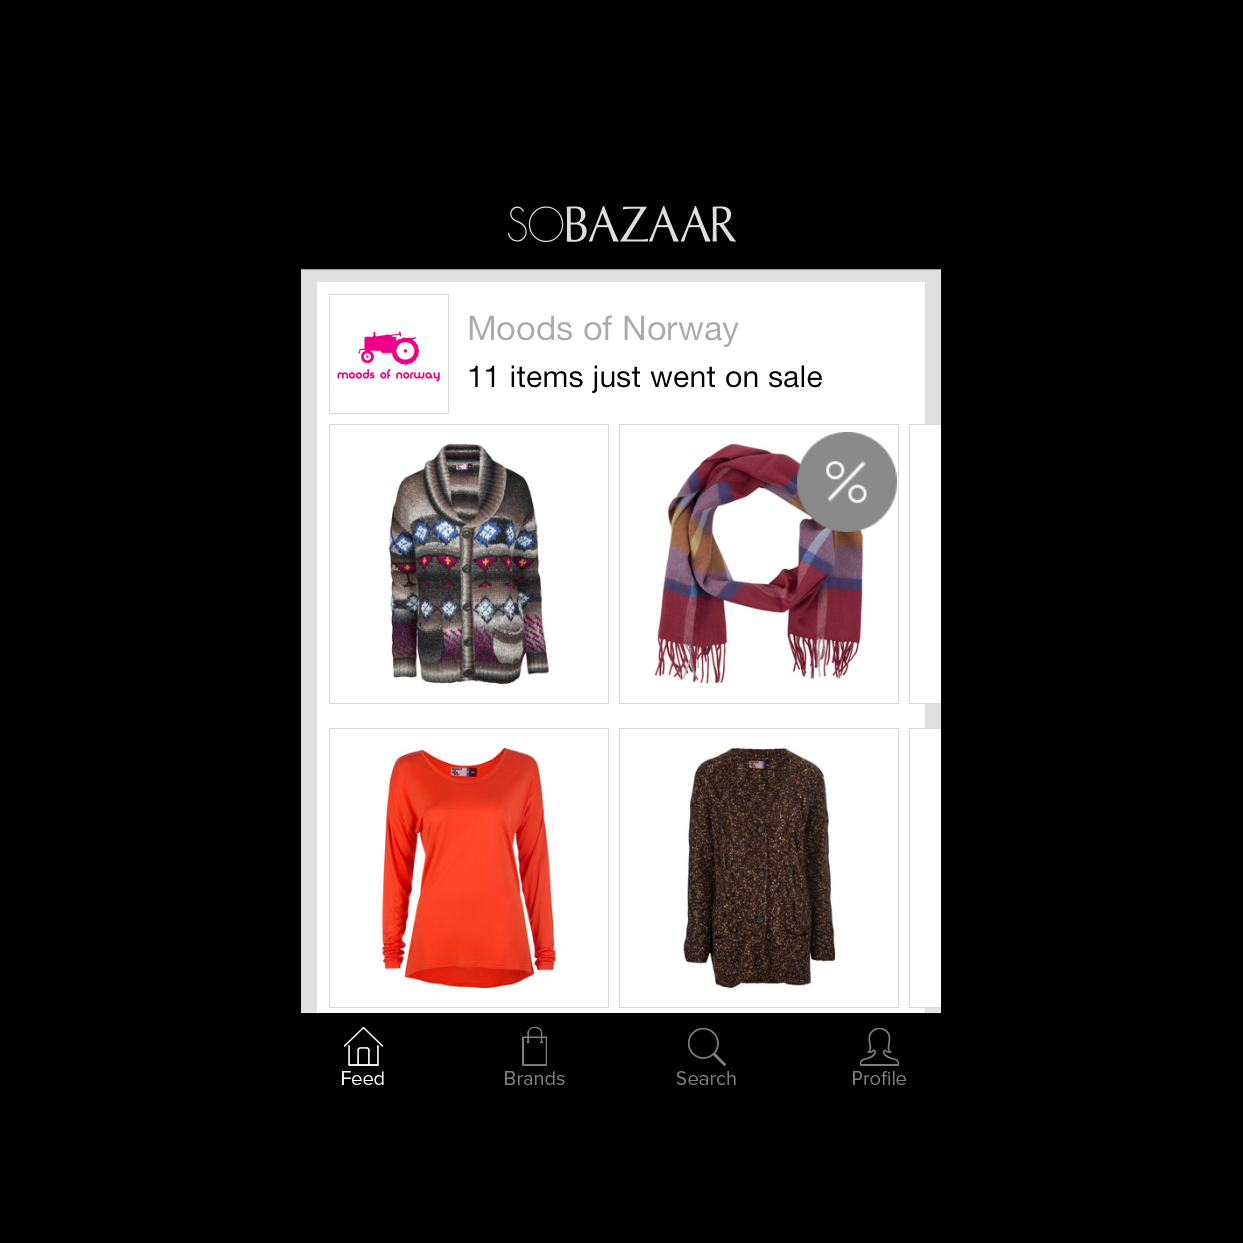
\includegraphics[height=1.5\linewidth]{image/sobazarsale.png}
		\end{minipage}
		\hspace{.02\linewidth}
		\begin{minipage}{.3\linewidth}
		  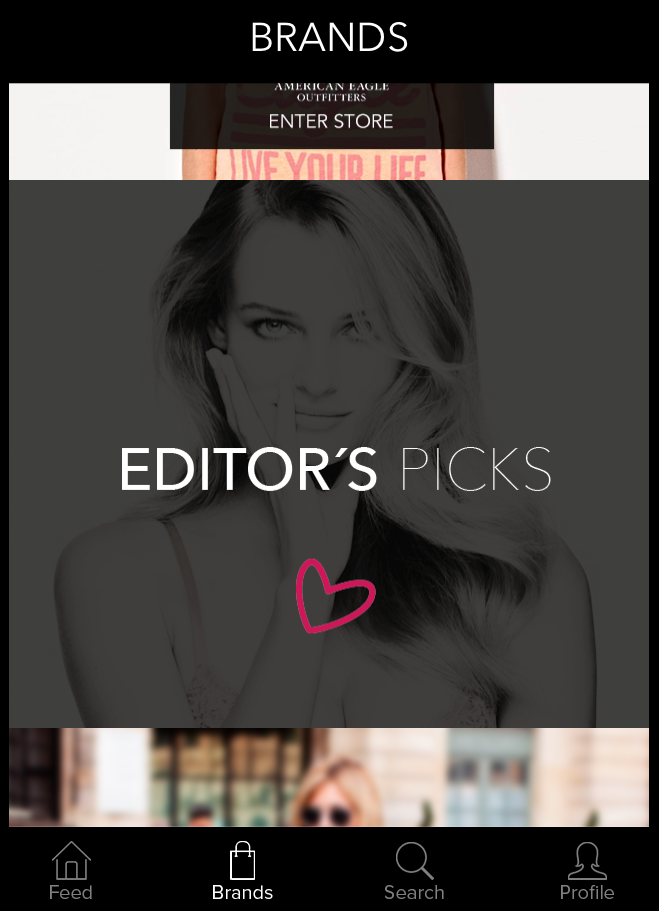
\includegraphics[height=1.5\linewidth]{image/sobazareditor.png}
		\end{minipage}
		\hspace{.02\linewidth}
		\begin{minipage}{.3\linewidth}
			  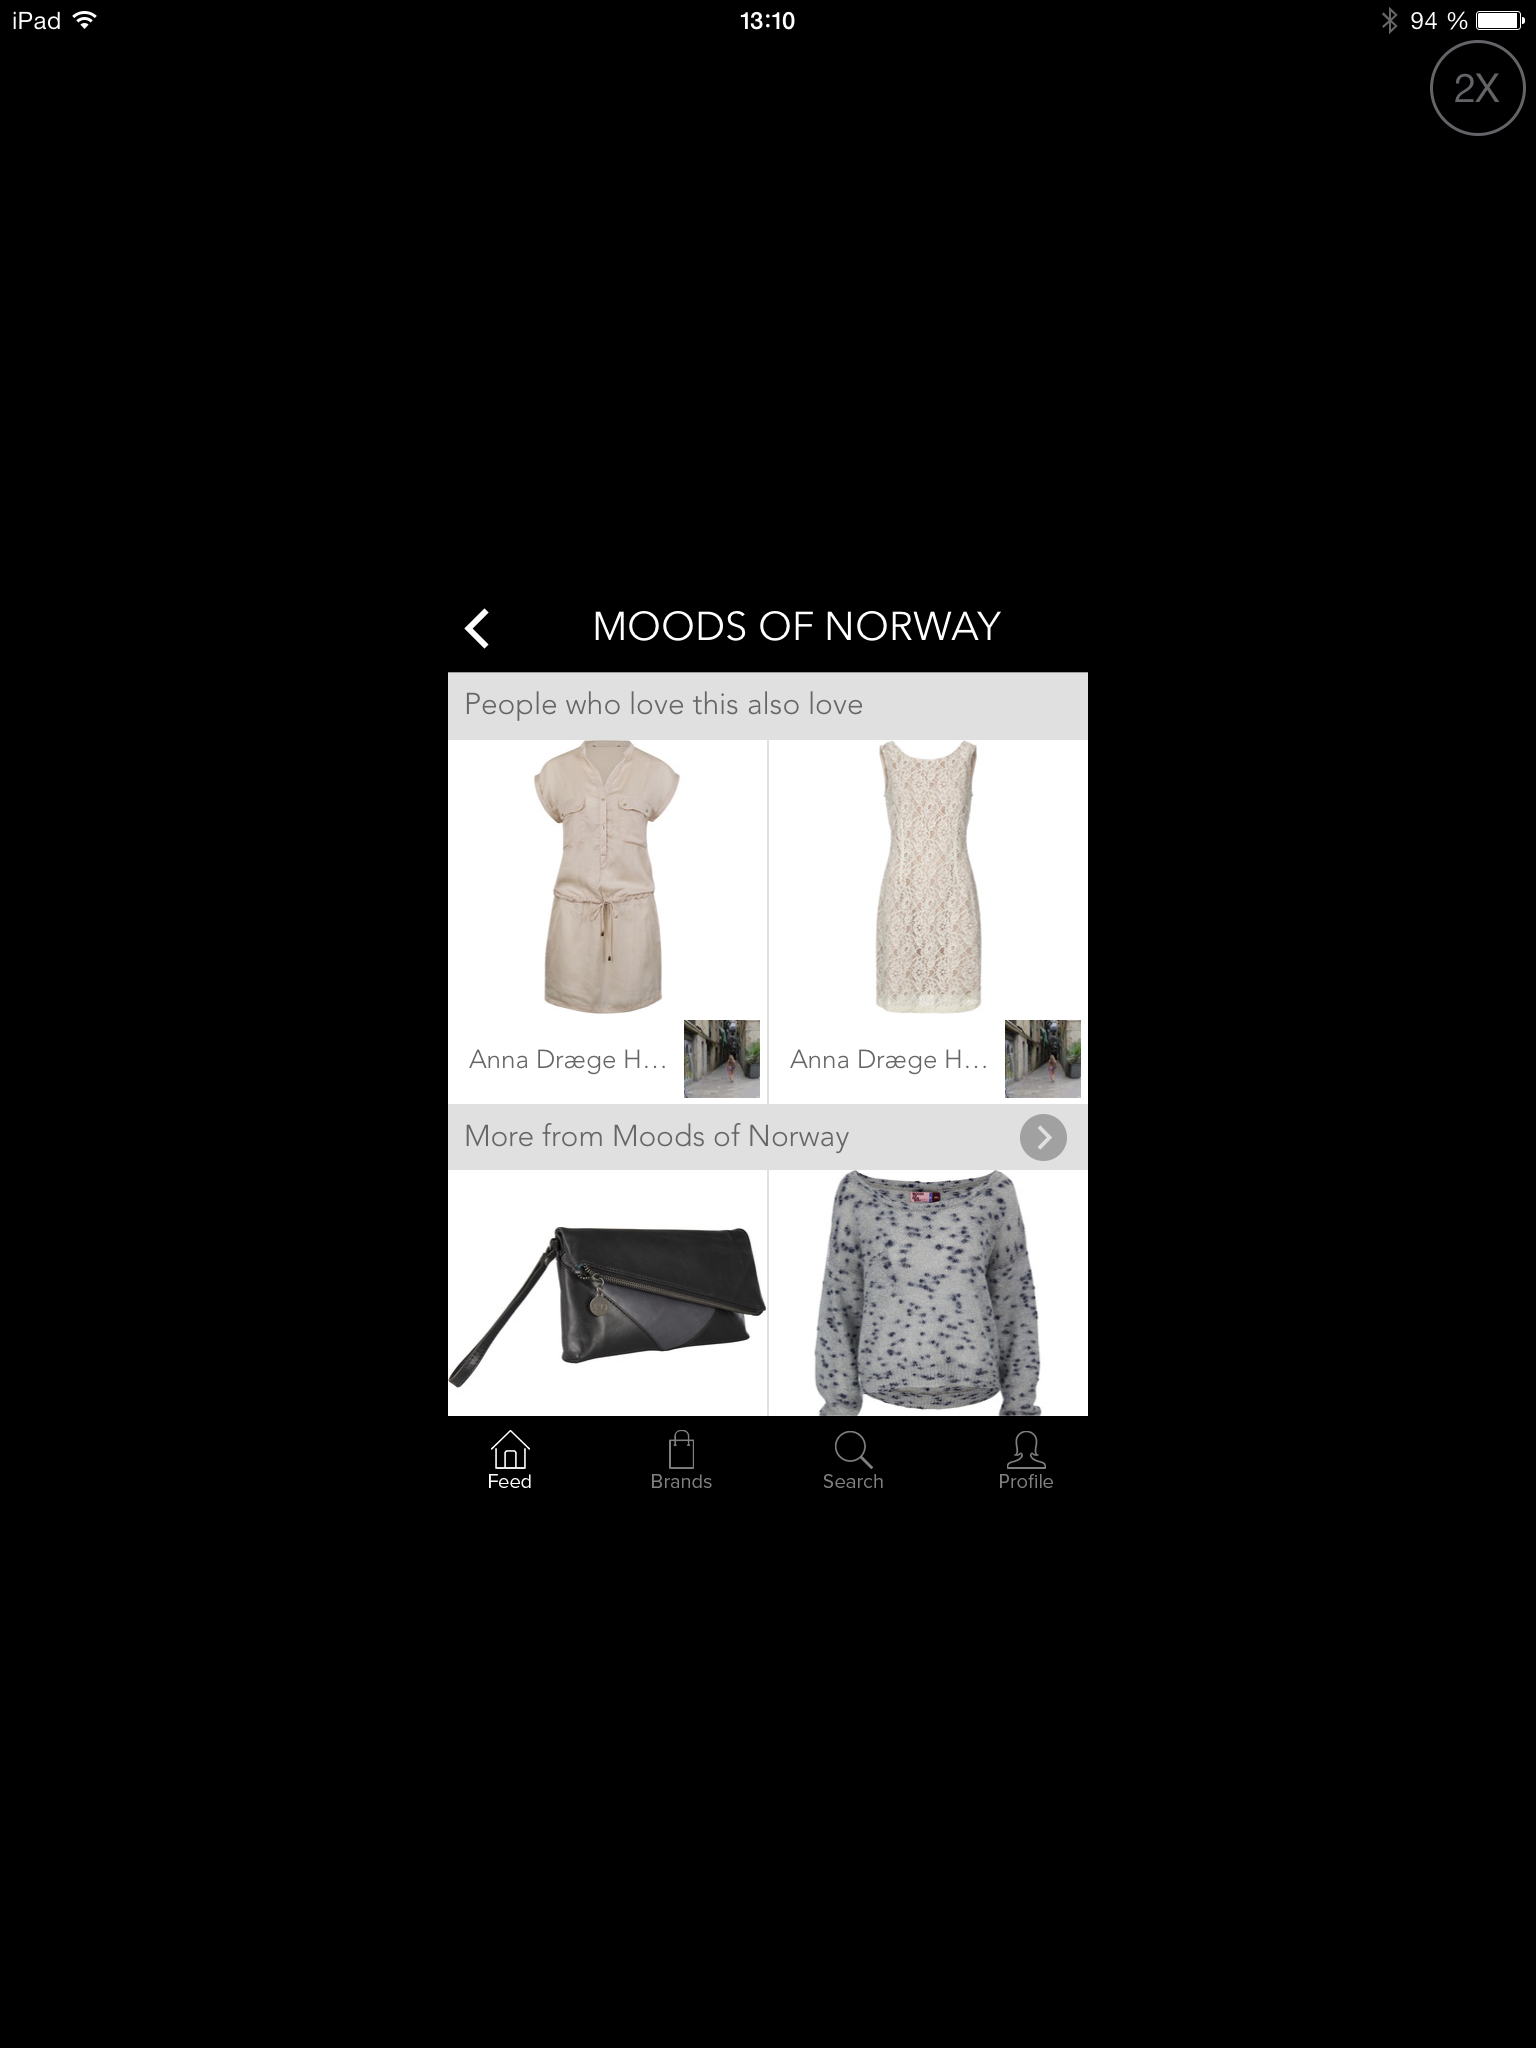
\includegraphics[height=1.5\linewidth]{image/sobazarrelated.png}
		\end{minipage}
		\caption[Sobazar screenshots - version 0.5.1]{Screenshots from the Sobazar Application. From the left to right: A newsfeed sale notification, editors picks and related product widgets from the product screen}
		\label{figure:sobazarfeed}
	\end{figure}

	
	The application is currently in a beta phase and is planned for a final release after the summer. 
	
% mtodo - før vi kan lære dette
    % 1. soBazar info
    % 2. sessions of events m eksempel

\marginpar{Not updated with the newest data}

\section{Data Cleaning}
    \marginpar{Some better way of saying this; Data Preprocessing, Data Prefiltering, something}
    The data from Sobazar came as is from the Sobazar database, with the exception that the data had been anonymised for privacy reasons.
    It contained therefore some unnecessary events.
    The data was therefore cleaned by removing events containing test environment flags such as: test environment and applications run from simulator.
    What was left after the cleaning data was mainly events triggered by the users, and no created during applications testing.

    %mtdo - why do we need data cleaning?

\section{Dataset Summary}
    The data from Sobazar is gathered based on the actions of the users in the application.
    When a user accesses a store or an item, the information regarding the user and the item is stored, this is often known as implicit feedback~\ref{sec:implicit}.
    Events such as purchasing an item and "wanting" and item is stored in the same manner, but can in many cases be considered as explicit feedback.

\subsection{Event Metadata}
    When an event is triggered a set of information is stored regarding the event.
    This data is used to make recommendations for the users though converting the implicit feedback to implicit ratings.

    %mtodo - vet vi hva dette er?

    \begin{table}[H]
        \centering
        \begin{tabular}{l l}
            \toprule
            Variable     & Explanation   \\ \midrule
            price             & The price of the item which triggered the event \\
            product\_id       & The id of the item which triggered the event \\
            storefront\_id    & The store id from which the item originated \\
            event\_id         & What kind of event was triggered~\tablefootnote{Complete list of the different types of events can be found in table~\ref{table:events}} \\
            event\_location   & The location of the user when the event was triggered \\
            ts                & Unix timestamp in milliseconds of when the event was triggered \\
            session           & Which session number the event belongs too~\tablefootnote{This value is added at a later time. For two events to end up in the same session, the event has to be triggered within a certain period of time, and both be after the same application started-flag} \\
            user\_id          & The unique id of the user who triggered the event \\
            \bottomrule
        \end{tabular}
        \label{table:eventData}
        \caption[Event Metadata]{Metadata collected from an event. The complete list can be found in table~\ref{table:completeEventData}}
    \end{table}

    %How much preference data?
    %Which events are interesting to look at?
% \subsection{Numbers}
    \begin{table}[H]
        \centering
        \begin{tabular}{l l}
            \toprule
            Attribute       & Count   \\ \midrule
            Unique users ids   & 1235           \\
            Unique item ids    & 3386           \\
            Unique brands      & 16             \\
            Purchases          & 1484           \\
            Wants              & 7726           \\
            Item Clicks        & 14036          \\
            \bottomrule
        \caption[Dataset summary]{Overview of the key figures in the Sobazar dataset}
        \label{table:datasetSummary}
        \end{tabular}
    \end{table}
    \marginpar{input the updated data when/if we get a new dump from Sobazar}

    % \begin{table}[H]
    %     \centering
    %     \begin{tabular}{l|l|l}
    %         Offer database length           & 7854   & ~ \\ \hline
    %         Event items length              & 4042   & ~ \\ \hline
    %         NonMatching values:             & 620    & ~ \\ \hline
    %         Items from Events not in Offer  & 7.89 \% & ~ \\
    %     \end{tabular}
    %     \caption[]{Items in events not in the actual offer database }
    % \end{table}

% \subsection{The Expected}
%     Event "app\_started", all have user\_id's
%     Event "app\_first\_started", all user\_id's are NULL
%     Event "user\_logged\_in", all have user\_id's... (assigned with login, event saved after login?)

% \subsection{The Strange}
%     NULL valued  for user\_id events: (Not all strange, but put together for readability)
%     facebook\_share\_changed

%     collection\_viewed  ignoring collection view-event as of now since the user\_id
%     is null. Could be valuable to use, though (30 000 events ignored) ...
%     potential workaround:
%         for each session do:
%             Filter all events on:
%                 session-ts-start to session-ts-end,
%                 allow: user\_id session-user-id and NULL
%                 Ip of user-session and ip of collection\_viewed
%                 storefront\_id's from session
%                     Populate collection\_viewed-user-id with session-user-id

%     Potential faulty user-id setting for ip-switch during a session, but expect few
%     occurrences of this

%     wantlist\_menu\_entry\_clicked
%     app\_became\_active

%     app\_first\_started
%     facebook\_login\_failed

%     > db.prod.distinct('event\_json.ipAddress').length
%     9033
%     > db.prod.distinct('event\_json.eventData.device\_id').length
%     2644
%     > db.prod.distinct('user\_id').length
%     1660

%     More devices than users, can't fill the blanks with device\_id

%     Q's:
%         app\_became\_active id's for better sessions?
%         store\_clicked vs. storefront\_clicked (23 vs. 19744)
%         API item-id's mapping to event product\_id's; how to map?


%     soBazar want to build a proper model.  Give input on how to build this model.
%     The supplier should know that an item is a jacket for instance.  Have something
%     to show on the 20. Should be better than what is already implemented.

\section{Graphs}
    % Price ranges of all items (groupings)
    % Item time on market TODO maybe not that interesting alone
    % Count for different events
    % Distinct events done on stores (shady)
    % peak online (slope-style) (events per day)
    % Price range of items in stores
    % count User eventes
    % user-item (how many items has a user "interacted" with)
    % Count of unique items in item db also in event db
    % Usable events regarding userid (events types with not null userid)
    % (Plotting locations)
    % unique Stores count for users

    % complex 3.Deg:
    %     count Sessions for users (aprox: sessioncount)TODO
    %     price span for user
    % complex 4.Deg:
    %     Stats for sessions:
    %         Timespann of sessions for users (avg, max, min)
    %         Events per session (avg, max, min)
    %         Item viewtime for user in session
    %         Stores visited per session
    %         revisit time of items for user
    %         relationship with view, want and purchase
    %         time of session over lifetime of app
    %         user preferred price in session

    % complex 5.Deg:
    %     Stats for global session stats:
    %         price vs view, want and purchase
    %         avg viewtime for an item (i know)
    %         Similarity of user favorite store, items viewed and items wanted?
    %         time of session over lifetime of app for all users (slope-style)

    % new:
    %     item timespan (first item interest - last item interest)
    % Blobs of smaller bubbles with eventid
    % Blobs for eventcount on stores with items items from stores (populate "storename" for "itemevents")
    % Show occurence of event after other event?
    % User stats: items, likes, intented purchased, events, session avg, max event, fequency
    % Find prices for stores: prize ranges

    % is viewing a item (with the possible, albeit unknown intent of consuming) really the same class of problems as actually consuming a item, and how does amount of looking map to amount of consumption?

    \begin{figure}[H]
        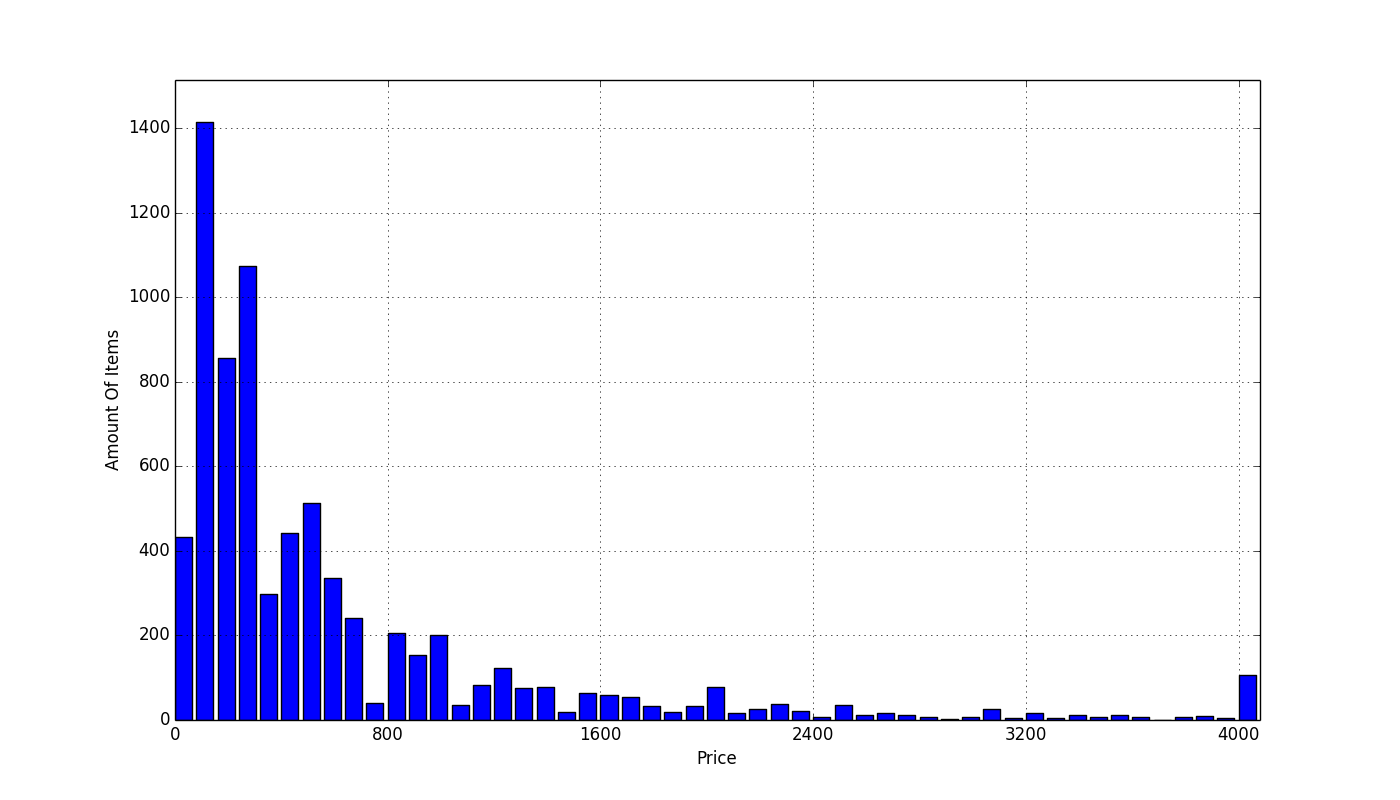
\includegraphics[width=5in]{image/priceDistribution.png}
        \centering
        \caption[Price distribution of items]{Here we see how them items are distributed on amount of items and price. The red bars indicates the amount of items with the belonging price.
        All items priced over 3 000 are put in the same bucket, and is the reason for the last spike we see at 3 000.
        We can see from this graph that the majority of the items are priced under 1 000 NOK}
        \label{figure:ratingdistr}
    \end{figure}

    %mtodo - better buckets to better capture the ranges
    %mtodo - ikke ha all teksten i captionen til figuren, ha det heller i vanlig tekst
    \marginpar{TODO - Make it pretty}
    \begin{figure}[H]
        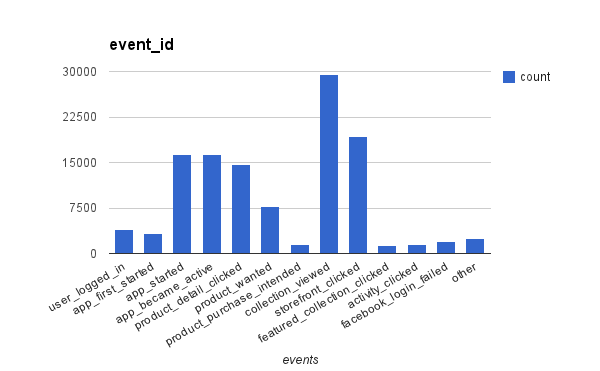
\includegraphics[width=5in]{image/event_id.png}
        \centering
        \caption[Count for different events]{This figure displays the count for each of the different events which can be triggered in the Sobazar application.
        The "collection\_viewed"-event and "storefront\_clicked"-event are the most common events to be triggered.
        Both of these types of events will send the user to an item overview, and indicates that many users browse the items through looking at the thumbnails rather than accessing the items, since the two named event types are gateways to collections of items, and if most of the users actually accessed most of the items the "product\_detail\_clicked", "product\_wanted" and "product\_purchase\_intended" would have had the majority of the events triggered.}
    \end{figure}
	\marginpar{TODO - Make it pretty}
    \begin{figure}[H]
        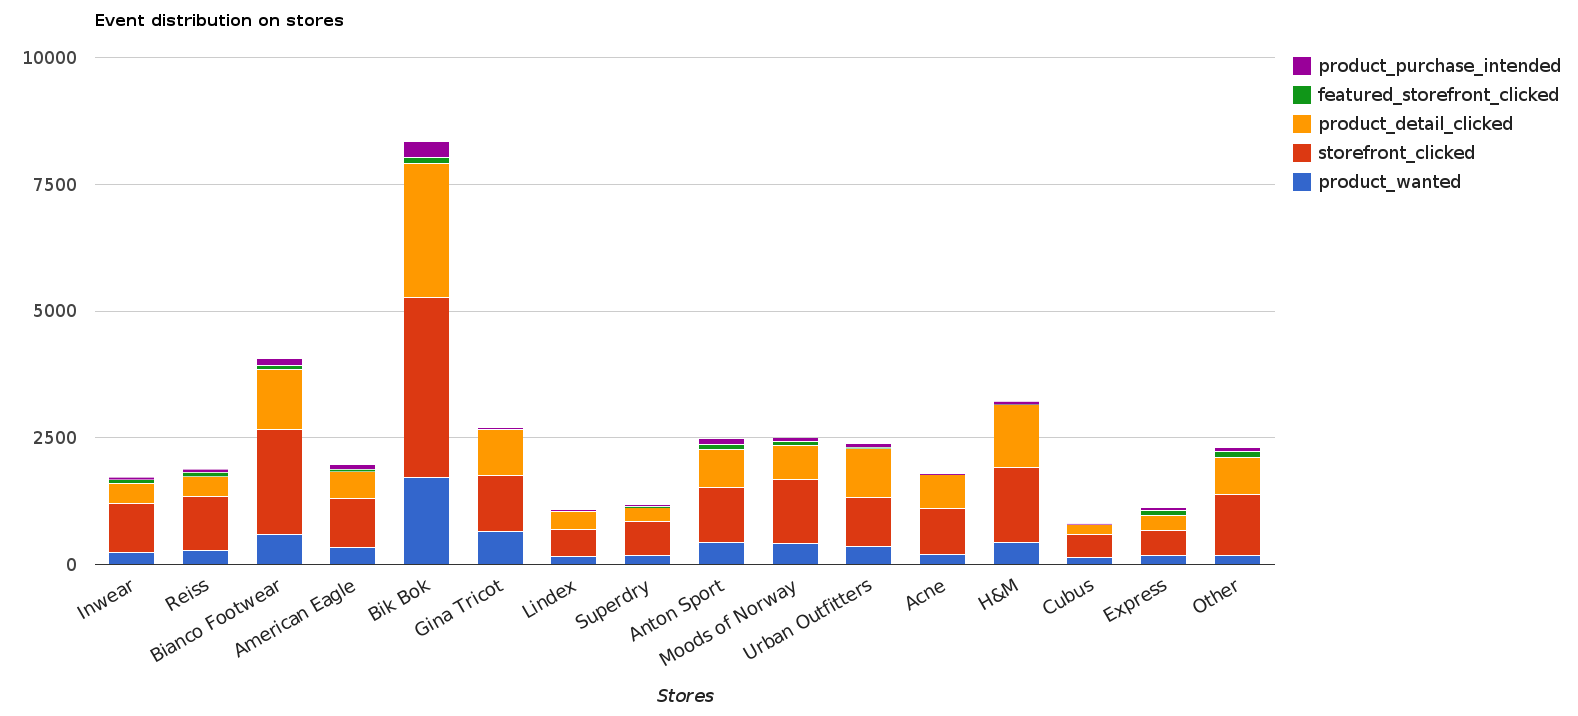
\includegraphics[width=5in]{image/event_distr.png}
        \centering
        \caption[Distribution of events on storefronts]{The events triggered in context with the different storefronts.
        The events are segmented to show the different event counts on the different storefronts, and stacked to show the complete count, to be able to clearly see how the events are distributed over the different stores.
        We can see that "Bik Bok" is the most popular store on all fields.
        One interesting find to take from this graph is the "storefront\_clicked" to the item interaction related events ("product\_detail\_clicked", "product\_wanted" and "product\_purchase\_intended") ratio.
        For instance "Bik Bok" has a much higher item interaction count than storefront access count, whereas stores such as "Reiss" and "Inwear" are mostly accessed and the items not interacted with.
        Different aspects affecting this might be price, style and item presentation.}
    \end{figure}

    % mtodo - session flytdiagram åpne app - se collection - se enkeltitem - kjøpe - skru av, piler mellom og shit

    % \begin{figure}[H]
    %     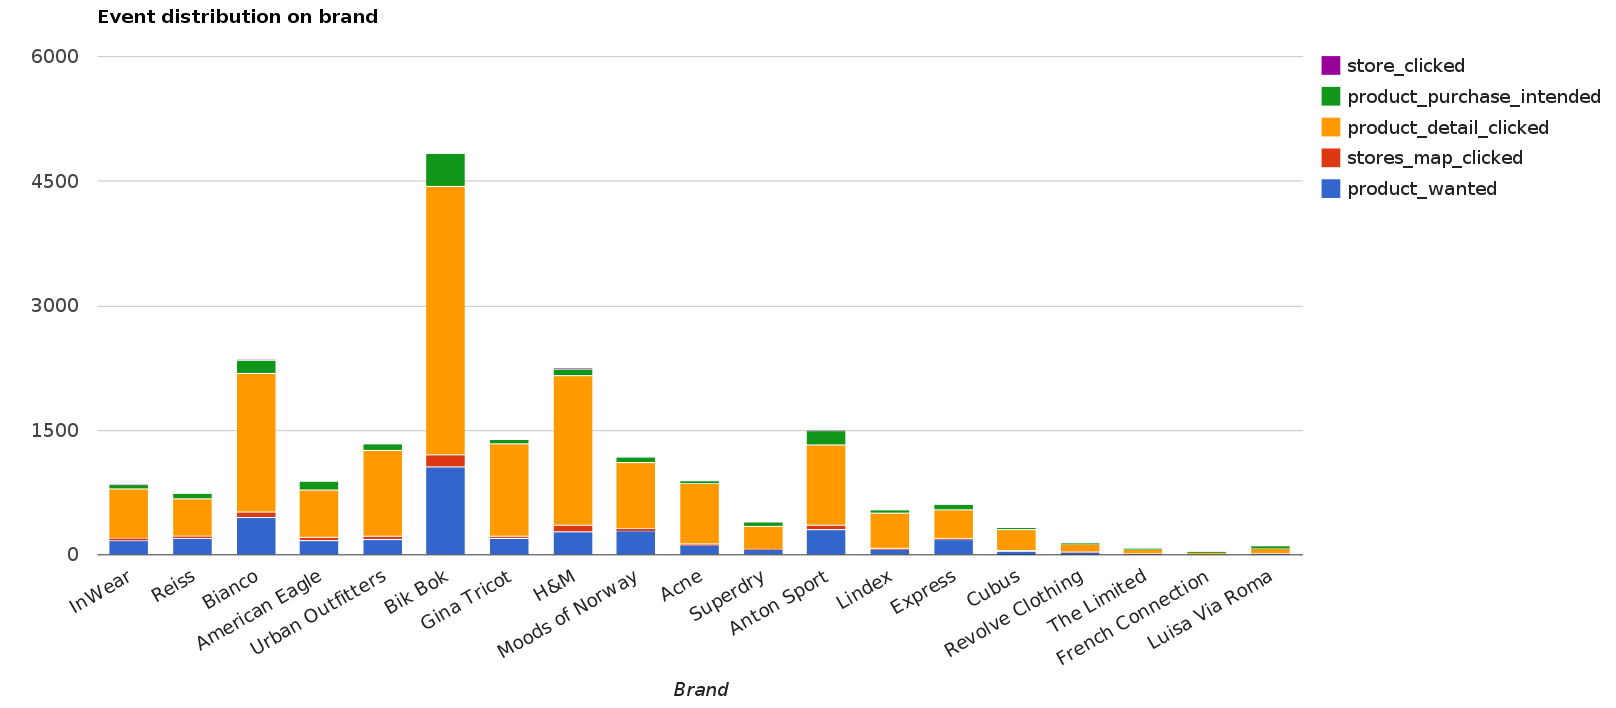
\includegraphics[width=5in]{image/brand_distr.png}
    %     \centering
    %     \caption[Distribution of events on brands]{This figure shows how the users are interacting with the different brands. }
    % \end{figure}

    \begin{figure}[H]
        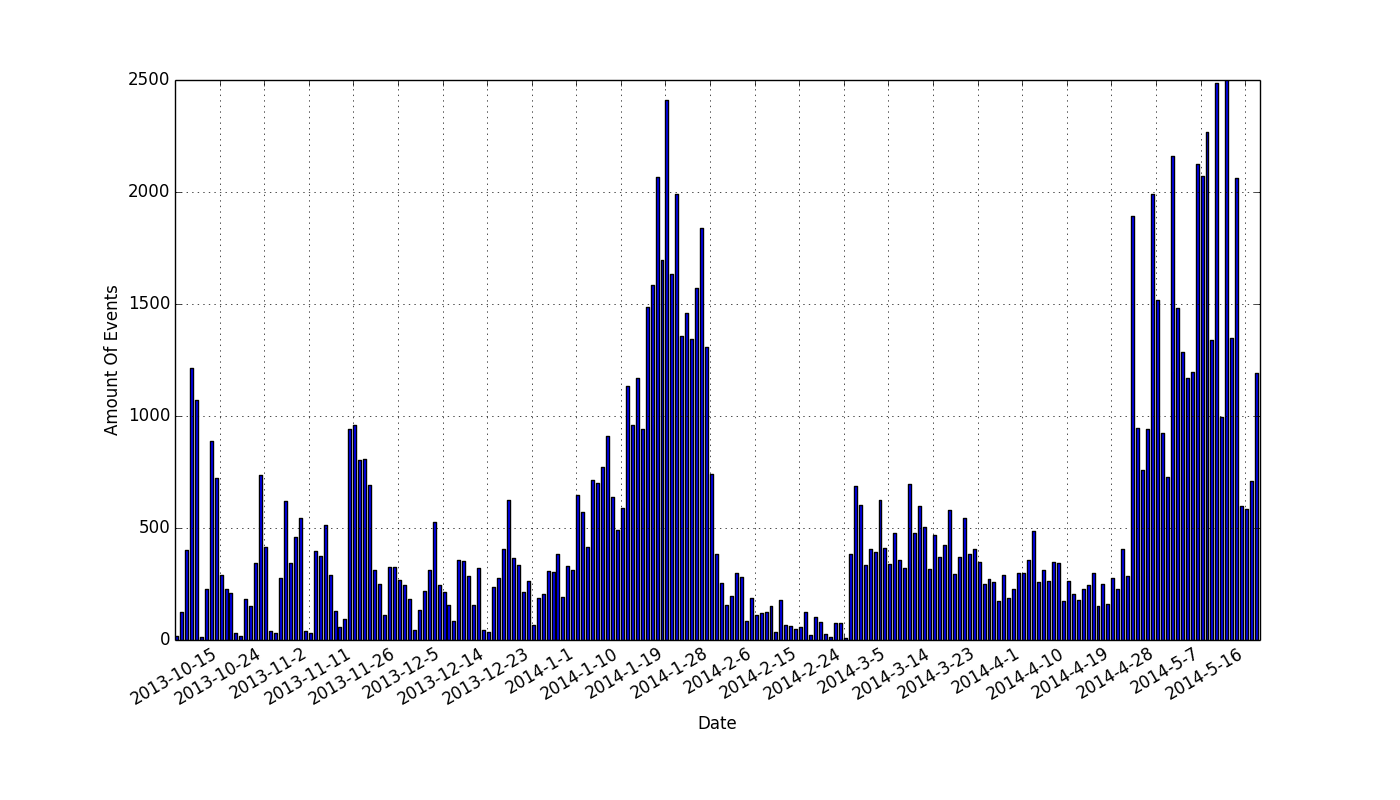
\includegraphics[width=5in]{image/eventsPerDay.png}
        \centering
        \caption[Distribution of events per day]{This figure shows the event distribution per day over the time period the events were stored.
        The spikes we see happens on a weekly basis, and is centered around the weekends.
        The larger spike from the start of January to the start of March might be due to increase in publicity or other outside factors.}
    \end{figure}

    \begin{figure}[H]
        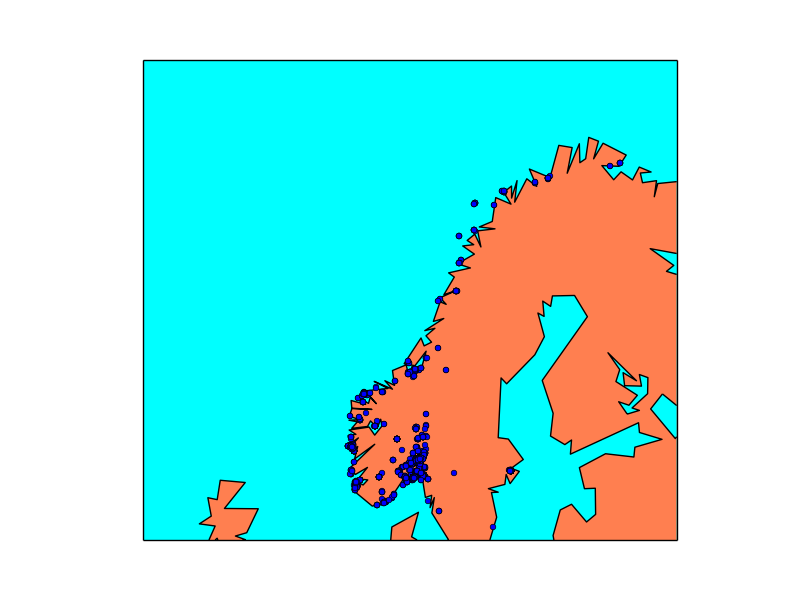
\includegraphics[width=5in]{image/simpleGeoPlot.png}
        \centering
        \caption[Simple plotting of event location]{This figure shows the location of the user at the time of the different event triggers.
        It is cropped to show events triggered in and around Norway.
        We can see that the majority of the users are located in and around Oslo.}
        \label{figure:croppedGeoplot}
    \end{figure}
	\marginpar{TODO: Cut at 70? (on the x-axis)}
    \begin{figure}[H]
        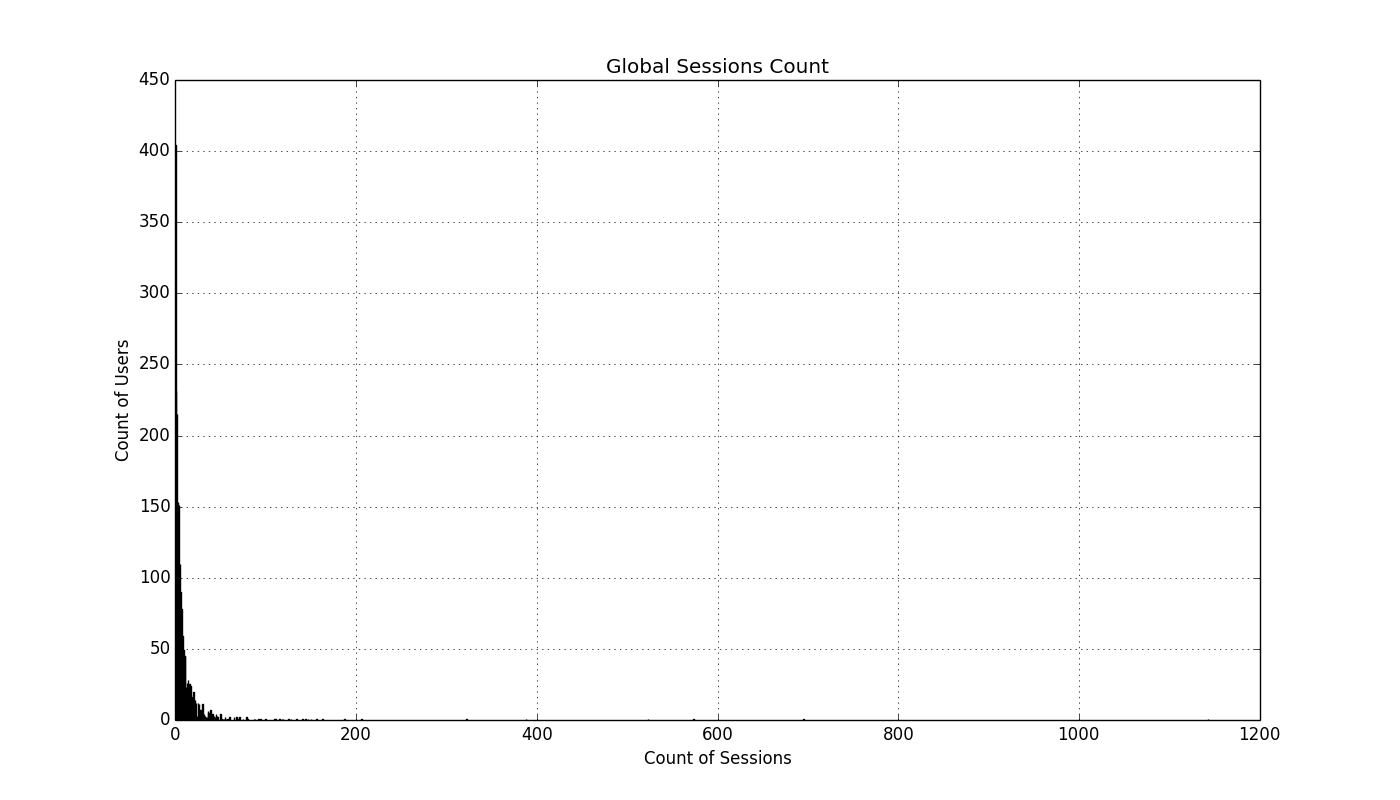
\includegraphics[width=5in]{image/sessionsCount.png}
        \centering
        \caption[Total max session count for the users]{The maximum number of sessions for each user grouped to show how the count of how many users has the different amount of sessions.
        The majority of the users of Sobazar has a session count of 20 and less.
        This means that they have not used the applications more than 20 separate times, over the time the data was collected.}
    \end{figure}

    % \begin{figure}[H]
    %     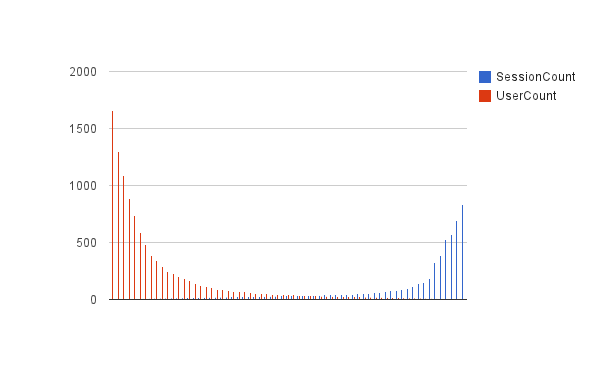
\includegraphics[width=5in]{image/global_sessioncount.png}
    %     \centering
    %     \caption[Count of sessions per user mapped with count of user with give
    %     session amount]{TODOsome awesome text}
    % \end{figure}
	\marginpar{TODO: cut on x-axis, make pretty}
    \begin{figure}[H]
        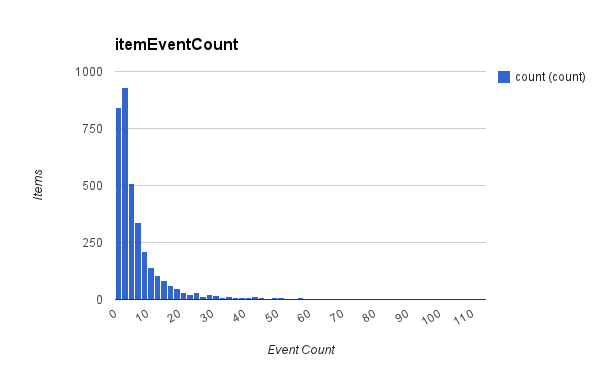
\includegraphics[width=5in]{image/item-event-count.png}
        \centering
        \caption[Count of events on each unique item]{This figure shows the unique count of events on each item in the Sobazar dataset.
        The majority of the items has only had a interaction count of 10 or less.
        Interaction count is "product\_detail\_clicked", "product\_wanted" and "product\_purchase\_intended".
        This means that there will not be more than 10 events for the majority of the items, which might lead to an issue when doing collaborative filtering on the data.
        When the majority of the events only has 10 events and there are over 4 000 items and 1 200 users, the probability that multiple users have interacted with similar items will be low.}
    \end{figure}

    %mtodo - update numbers
	\marginpar{First to last event in days/weeks not minutes, remove text on a-axis (only confusing). Why is this important, clearify text, what can we learn from the plots?}
    \begin{figure}[H]
        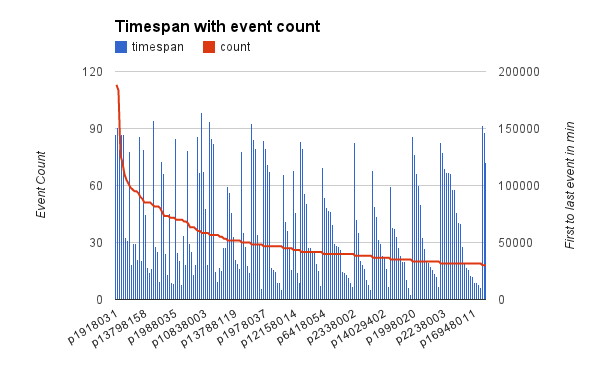
\includegraphics[width=5in]{image/item-timespan-event-count.png}
        \centering
        \caption[Life time of items mapped with event count]{This figure shows the total life span of each item mapped together with the amount of events triggered on them.
        The life span of an item is the time since the first event on the item till the last event on the item.
        Time is shown in minutes, so the longest time span of an item is about 105 days, which is close to the time span of the events gathered from Sobazar.
        Even though an item has had a long time span does not mean that the item has been of measurable interest to the users in the Sobazar application.}
        \label{figure:itemTimeSpanEventCount}
    \end{figure}

    % mtodo - si noe om hvorfor ikke? jeg vil vel påstå at dette sier no om viktihet av "nyhetsverdi" for item'et, og ville derfor trodd dette var relevant info?
	\marginpar{TODO: Change x axis from minutes to days (or preferably weeks). Does this give us any hints regarding time decay factors?}
    \begin{figure}[H]
        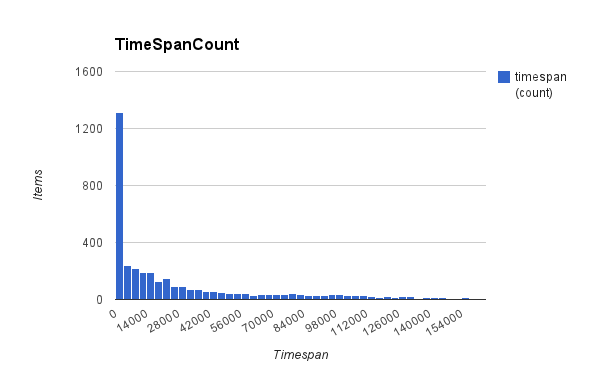
\includegraphics[width=5in]{image/time-span-count.png}
        \centering
        \caption[Count of the different time spans of the items]{This figure shows the count of items which has the different time spans.
        The numbers on the x-axis is in minutes.
        This figure makes it clearer than figure~\ref{figure:itemTimeSpanEventCount} how long the majority of the the items have lived.
        Most of the items has a time span of less than 14 000 minutes, which is less than 10 days.}
    \end{figure}

    % hvorfor? er det pga:
        % a) pga veldig få events
        % b) pga kort levetid for item i datasettet
        % c) fordi det bare hadde 10 dagers "nyhetsverdi"?
	\marginpar{TODO - Use seconds?}
    \begin{figure}[H]
        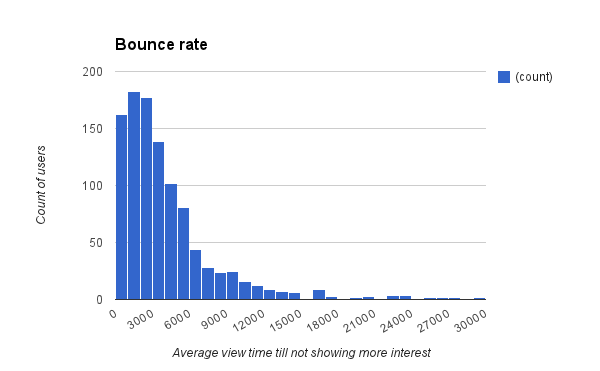
\includegraphics[width=5in]{image/bounceRate.png}
        \centering
        \caption[View time before leaving an item (Bounce Rate)]{This figure shows the time the users use before not taking any more action towards the item (purchase it or want it).
        The time is in milliseconds.
        The majority of the users have a view time of less than 6 000 milliseconds before they moves on to another item.}
        \label{figure:bounceRate}
    \end{figure}

    % mtodo - hva betyr dette for oss? ha det i seconds, lol

    \begin{figure}[H]
        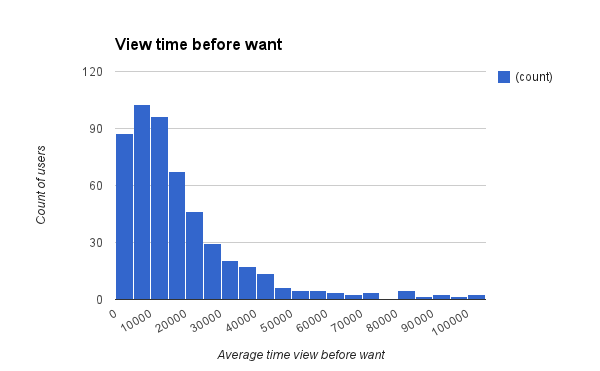
\includegraphics[width=5in]{image/viewBeforeWant.png}
        \centering
        \caption[View time before wanting an item]{This figure shows the time the users use before wanting the currently viewed item.
        The time is in milliseconds.
        The majority of the users have a view time of less than 30 000 milliseconds before they want the currently viewed item.}
        \label{figure:viewWant}
    \end{figure}

    \begin{figure}[H]
        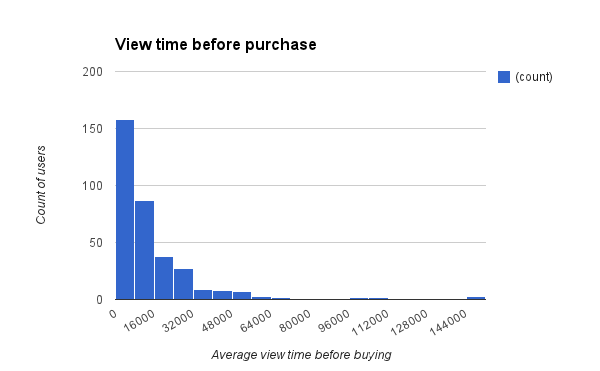
\includegraphics[width=5in]{image/viewBeforePurchase.png}
        \centering
        \caption[View time before purchasing an item]{This figure shows the time the users use before purchasing the currently viewed item.
        The time is in milliseconds.
        The majority of the users have a view time of less than 32 000 milliseconds before they decide to buy the currently viewed item.}
        \label{figure:viewBuy}
    \end{figure}

\subsection{About the view time before tanking an action}
    As seen from the figures~\ref{figure:bounceRate}, ~\ref{figure:viewWant} and~\ref{figure:viewBuy}, the bounce rate is quite small compared to the time it takes for a user to decide to want or buy an item.
    This could be used as an indication of negative feedback, but since there is no explicit feedback to to test this, it might lead to rating an item negatively when the user in fact would like to rate it positively.


    %mtodo - masse fin info, men diskuter!
        % hva betyr det for oss?
        % hvordan kan data-pakket brukes av systemet?
        % dette er hands-on!
        % mange fine figurer uten konkrete beskrivelser og refereanser i teksten
        % prøv heller å lage gode forklaringer til fiugurene i teksten så referer deretter

\section{Session Findings}
\marginpar{Something about session findings perhaps}

    % mtodo - fix caption and section :P
	\marginpar{TODO: Remove all arrows with less than e.g. 50 events}
    \begin{figure}[H]
        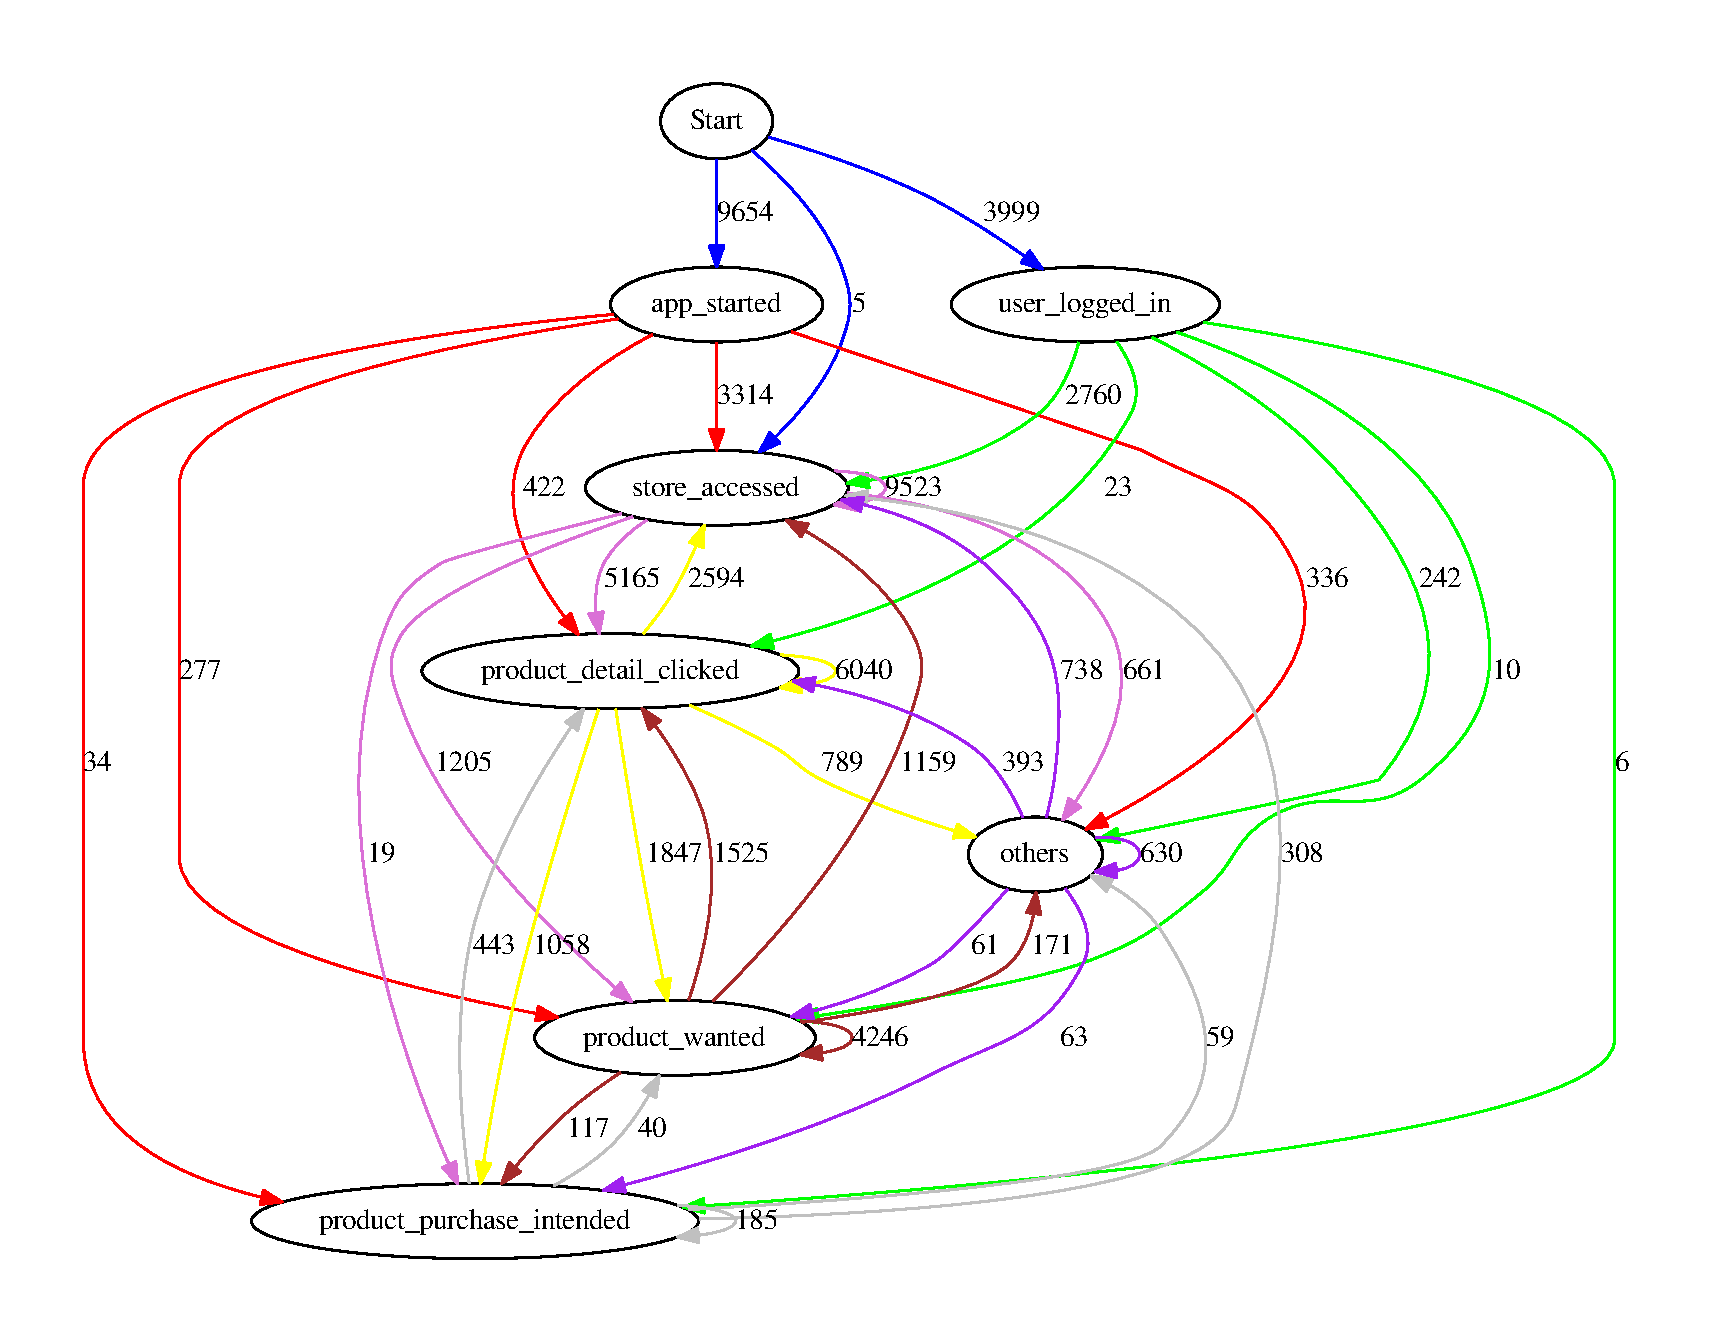
\includegraphics[width=5in]{image/statesInteractionTrue-gvfile.pdf}
        \centering
        \caption[Minimized states in session and how they interact]{A minimized view of the different states of the system and how they interact with each other.}
        \label{figure:minStatesInteractions}
    \end{figure}

    \begin{figure}[H]
        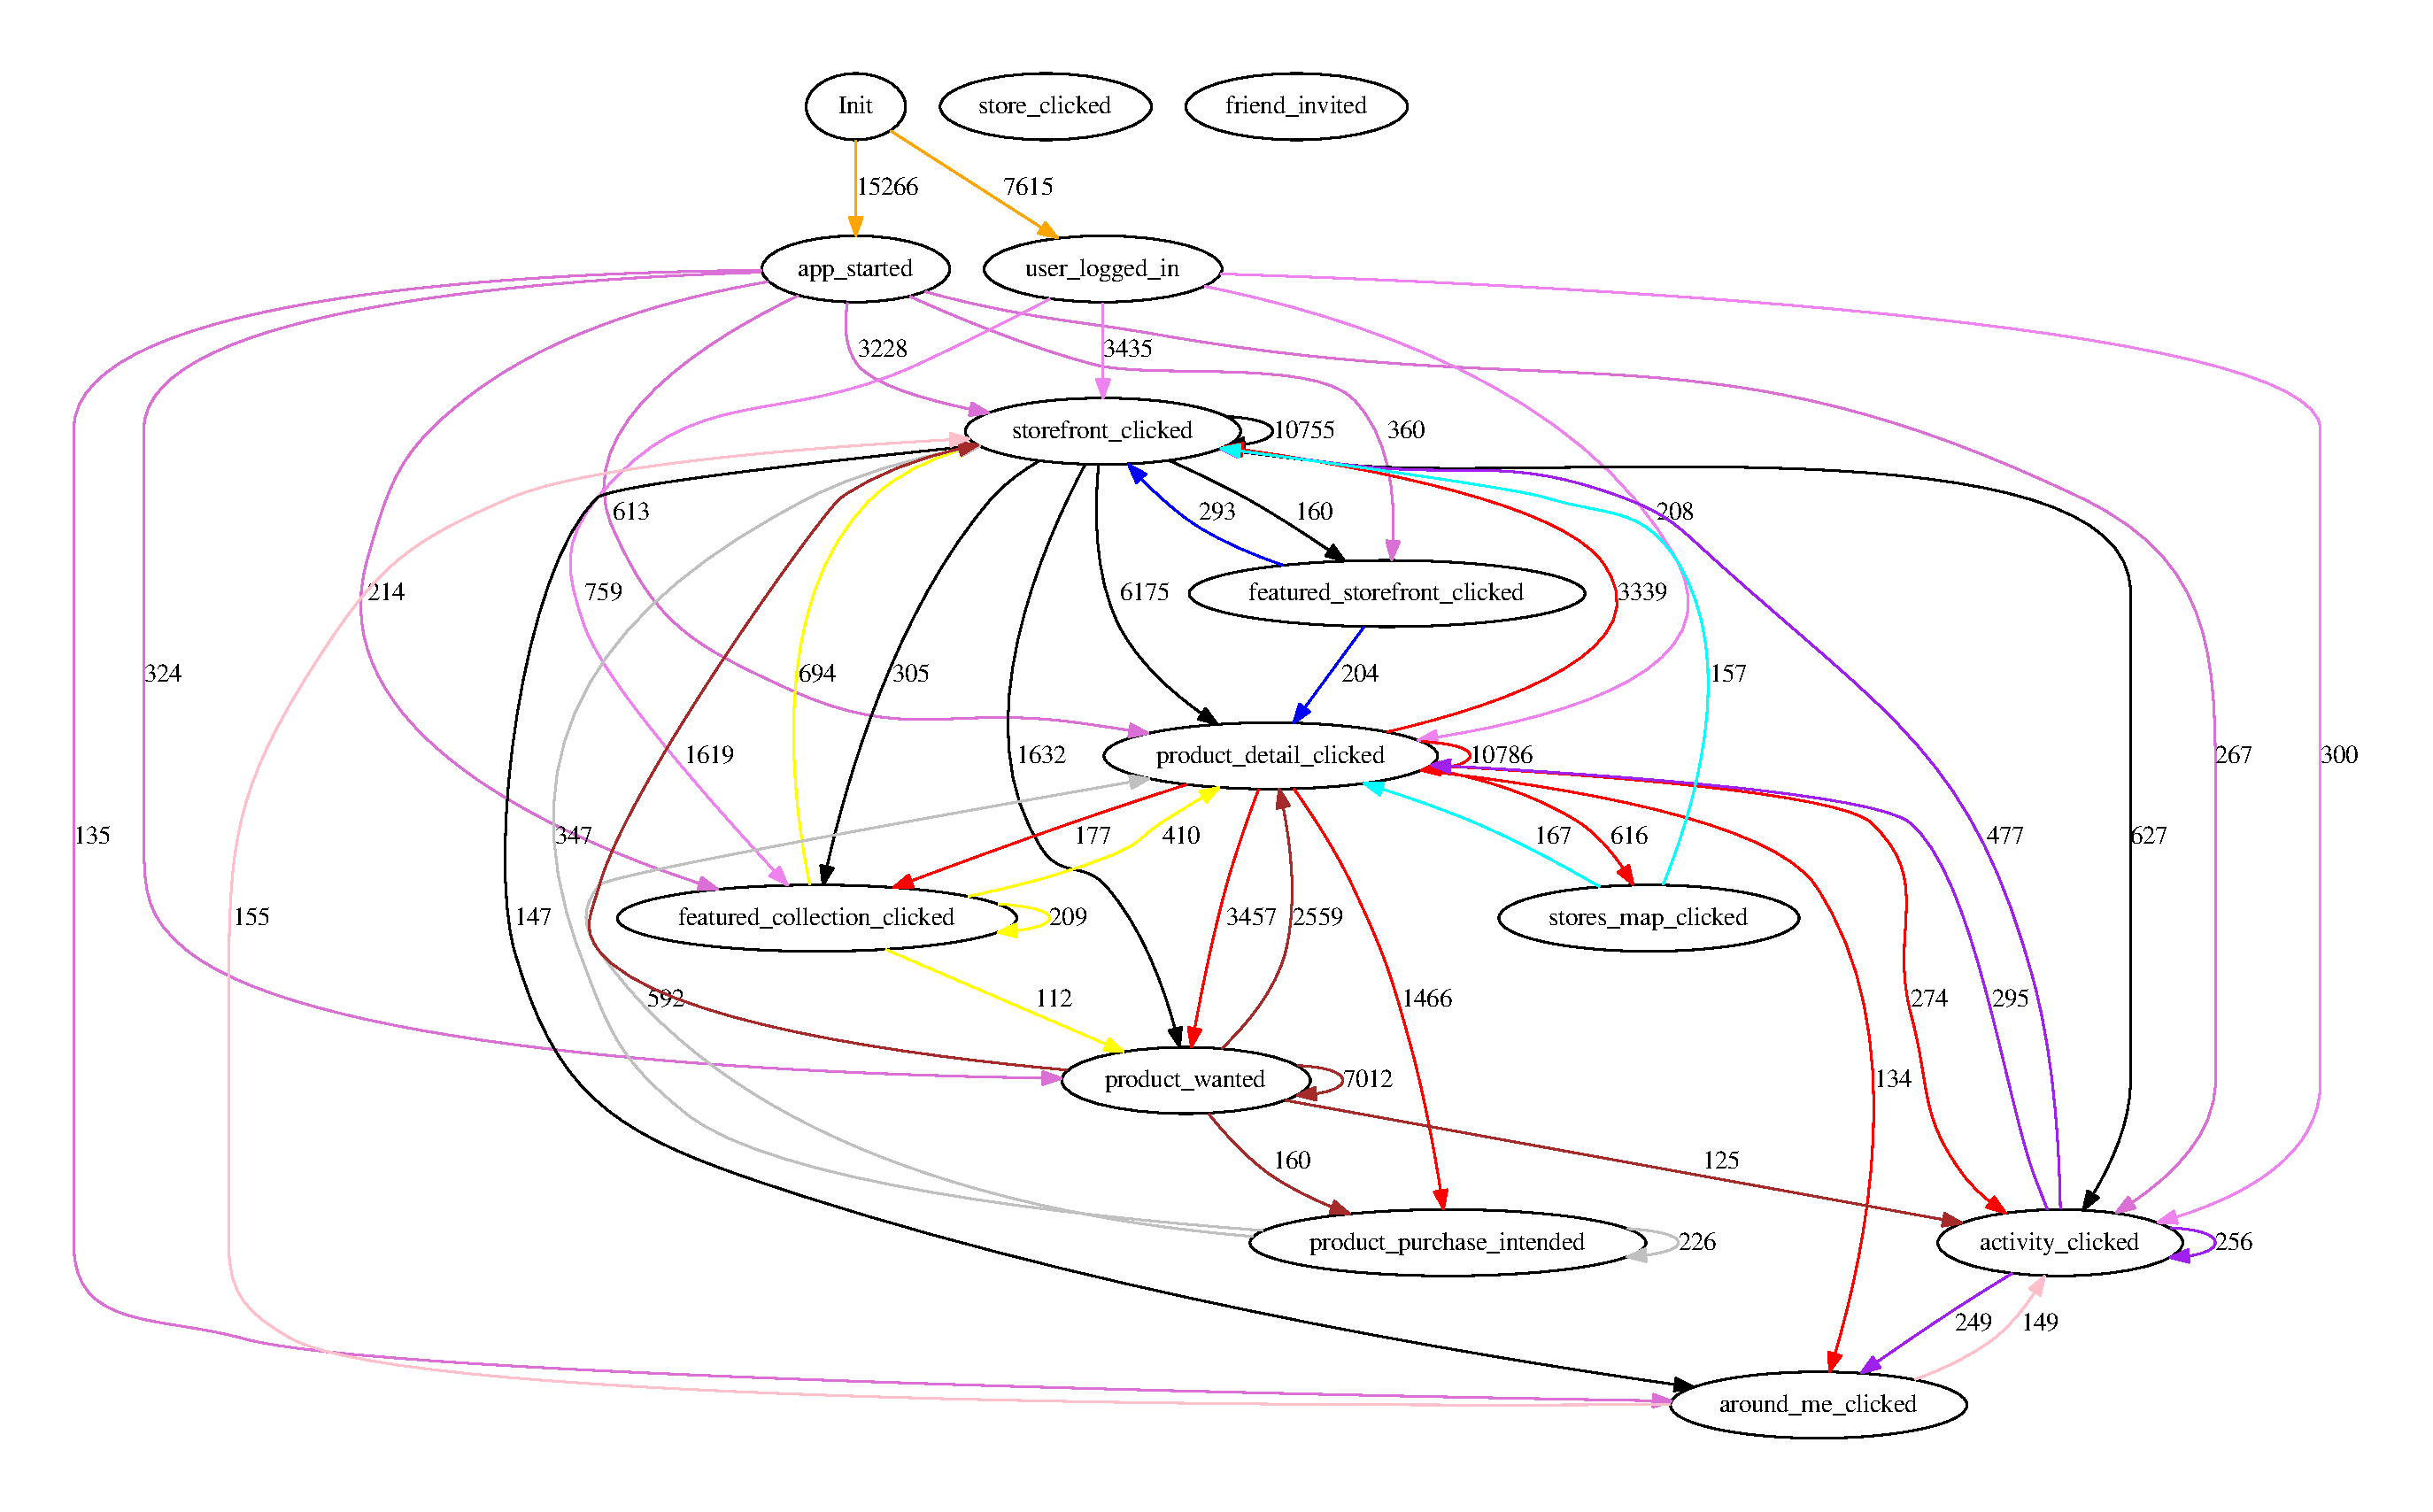
\includegraphics[width=5in]{image/statesInteractionFalse-gvfile.pdf}
        \centering
        \caption[States in session and how they interact]{The different states of the system and how they interact with each other.}
        \label{figure:statesInteractions}
    \end{figure}

    \marginpar{This is way too much information. Consider adding a threshold in
    order to reduce number of arrows}

    % mtodo - fix lol
    \marginpar{Will be moved to appendices}
%     Init Hypothesis:
%     Two users with similar session habits and similar product accessing pattern
%     have a stronger correlation to one-another than two users with just similar
%     product interests.


%     'product\_purchase\_intended' (user pushed to the product web store) shows a
%     wider specter of information about the product, including additional colors,
%     images and colors.  For some it might be natural to explore the item there
%     before "wanting" it. Making both

%     "product\_purchase\_intended" $\Rightarrow$ "product\_wanted"

%     and

%     "product\_purchase\_intended" $\notimplies$ "product\_wanted"

%     produce valuable information.

%     Must make different rules for the different stores:
%     "Bik Bok", "Cubus", "Gina Trik", "H\&M", "Bianco" has a broad specter of extra
%     functions inside the web store, whereas others might not, only shows the
%     product and a add to chart button.  This might divide the use pattern of the
%     users into a:

%     "product\_detail\_clicked" $\Rightarrow$ "product\_purchase\_intended" $\Rightarrow$ "product\_wanted"

%     "product\_detail\_clicked" $\Rightarrow$ "product\_purchase\_intended" $\notimplies$ "product\_wanted",

%     and

%     "product\_detail\_clicked" $\Rightarrow$ "product\_wanted"

%     based on the store accessed.

%     Use this to make a "rule set" with a probability.
%     Then again use this to recommend items for the users with that given
%     probability.

%     Find a "most popular session"-pattern
%     Find a "most likely to come after"-pattern

%     Session issues:
%     Once in a blue moon a user will do a "product action" (purchase,want,details)
%     without having a previous frontstore-access event. Which leads to unknown
%     store-id of the item.

%     Issue is most probably from missing user-id in collection\_viewed, and a user
%     checks out an item from there. It is not possible to be 100\% sure which user
%     access the item from the collection\_viewed event, so this event is therefor
%     not integrated into the session-stack.
